\chapter{Προγενέστερη έρευνα στο πεδίο} \label{ch:state-of-the-art}
\markboth{Προγενέστερη έρευνα στο πεδίο}{}

Για πολλά χρόνια οι άνθρωποι προσπαθούσαν να βρουν λύσεις που θα βελτίωναν την καθημερινότητα των ατόμων με μειωμένη όραση. Ο κύριος στόχος κάθε τέτοιας προσπάθειας ήταν να καταστήσουν πιο ασφαλή την πλοήγηση του χρήστη στον χώρο και παράλληλα να αυξήσουν την ταχύτητα με την οποία ο τυφλός χρήστης λαμβάνει αποφάσεις κατά τη διάρκεια της πλοήγησής του. Στο κεφάλαιο αυτό γίνεται μια αναδρομή, ξεκινώντας από τις κλασικές μεθόδους πλοήγησης των ατόμων με μειωμένη όραση μέχρι και τις πιο σύγχρονες ηλεκτρονικές συσκευές υποβοήθησης ταξιδιού (ETAs). Επιπλέον, παρουσιάζεται η τρέχουσα τάση στο σχετικό ερευνητικό πεδίο και παρατίθενται οι διάφορες κατηγορίες των συστημάτων υποβοήθησης πλοήγησης.

\section{Βοηθητικά μέσα υποστήριξης ατόμων με μειωμένη όραση}
Εδώ και εκατοντάδες χρόνια οι άνθρωποι χρησιμοποιούσαν διάφορα μέσα με σκοπό την καθοδήγηση των ατόμων με μειωμένη όραση. Τα πιο διαδεδομένα και ευρέως αποδεκτά από την κοινότητα των τυφλών είναι το λευκό μπαστούνι και ο σκύλος οδηγός \cite{social_sciences_libguides_nodate}. Τις τελευταίες δεκαετίες, μετά την ραγδαία άνοδο της τεχνολογίας, ήρθαν στο προσκήνιο νέες συσκευές υποβοήθησης πλοήγησης που "σκανάρουν" το εξωτερικό περιβάλλον και μεταδίδουν την πληροφορία αυτή στον τυφλό μέσω ηχητικών ή απτικών σημάτων.
\subsection{Συμβατικά μέσα καθοδήγησης}
Πρόκειται για τα μέσα που χρησιμοποιούνται κατά κόρον από τα άτομα με περιορισμένη όραση. Τα μέσα αυτά έχουν αποδειχθεί πολύ χρήσιμα στην καθημερινότητα των τυφλών, έχουν κερδίσει την εμπιστοσύνη της κοινότητας αυτής, αλλά πολύ συχνά η περιορισμένη ελευθερία κινήσεων που επιτρέπουν ή το κόστος τους αποτελούν ανασταλτικούς παράγοντες για την απόκτησή τους.
\subsubsection{Λευκό μπαστούνι}
Το λευκό μπαστούνι είναι ίσως το πιο διαδεδομένο μέσο καθοδήγησης των τυφλών. Προσφέρει αυτονομία και αίσθηση ασφάλειας στον χρήστη, καθώς του επιτρέπει να σκανάρει τον περιβάλλοντα χώρο και να εντοπίζει τυχόν εμπόδια ή επιφάνειες προσανατολισμού, με περιορισμένο ωστόσο εύρος κινήσεων. Παράλληλα, η χρήση του επιτρέπει στους υπόλοιπους περαστικούς να αναγνωρίσουν την ιδιότητα του τυφλού και συνεπώς να είναι πιο προσεκτικοί. Το λευκό του χρώμα έχει νομοθετηθεί και αποτελεί ένδειξη ότι το άτομο που το κρατάει έχει προβλήματα όρασης.
\begin{table}[H]
    \centering
    \begin{tabular}{|c|c|}
        \hline
        Θετικά & Αρνητικά \\
        \hline
        \hline
        Εύκολη χρήση & Περιορισμένο εύρος κινήσεων \\
        Φορητό & Αδυναμία αναγνώρισης του είδους του εμποδίου\\
        Χαμηλό κόστος & \\ 
        \hline
    \end{tabular}
    \caption{Λευκό μπαστούνι, θετικά και αρνητικά}
    \label{tab:white-cane}
\end{table}

\begin{figure}[H]
    \centering
    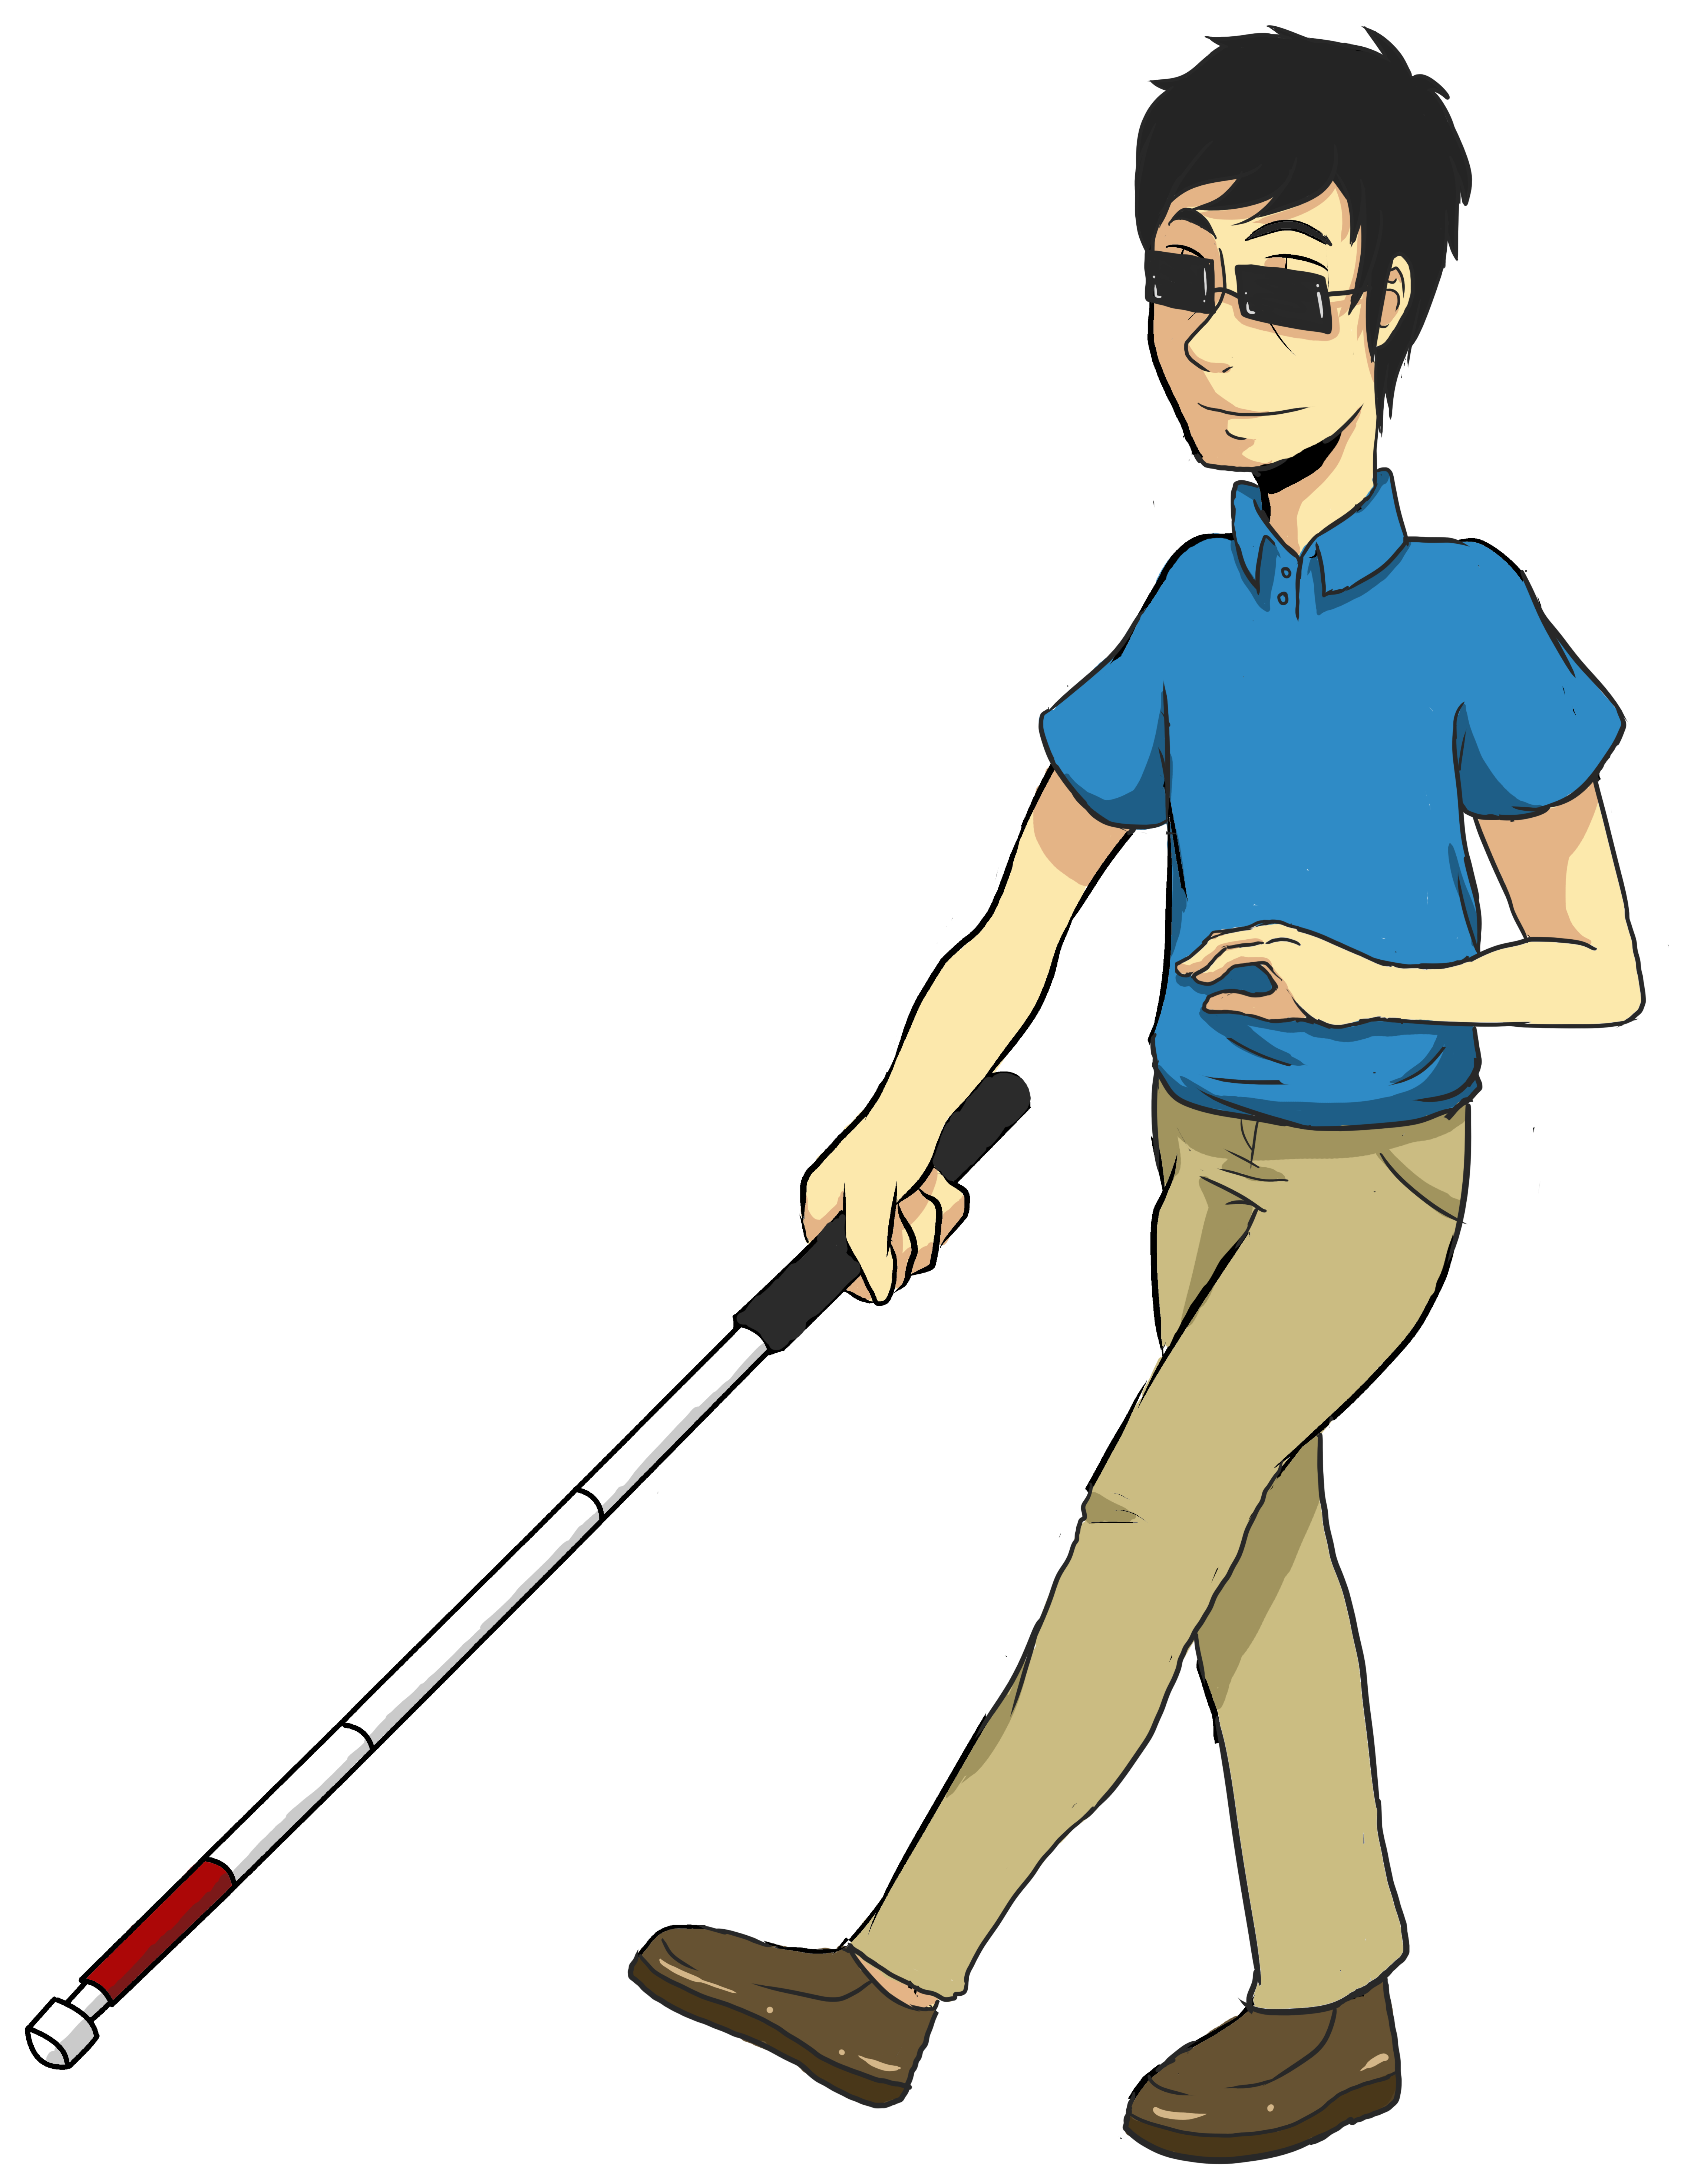
\includegraphics[width=0.4\textwidth]{images/white_cane_use.png}
    \caption{Παράδειγμα χρήσης λευκού μπαστουνιού}
    \label{fig:white-cane-use}
\end{figure}

\subsubsection{Σκύλος οδηγός}
Για πολλούς χρήστες με προβλήματα όρασης ο σκύλος οδηγός αποτελεί την καλύτερη λύση, αφού συνδυάζει την αίσθηση της ασφάλειας στην μετακίνηση με την αίσθηση της συντροφικότητας. Ο σκύλος οδηγός είναι εκπαιδευμένος να καθοδηγεί τον τυφλό με ασφάλεια, να αποφεύγει εμπόδια και να εντοπίζει στοιχεία όπως διαβάσεις, πόρτες, σκάλες, ταμεία και μέσα μαζικής μεταφοράς (π.χ., την είσοδο στο λεωφορείο). Η καθοδήγηση από έναν σκύλο οδηγό είναι πιο γρήγορη σε σύγκριση με το λευκό μπαστούνι, προσφέροντας μεγαλύτερη αυτονομία στον χρήστη. Παρ' όλα αυτά η εκπαίδευση ενός σκύλου οδηγού διαρκεί αρκετούς μήνες και απαιτεί αρκετούς οικονομικούς πόρους.
\begin{table}[H]
    \centering
    \begin{tabular}{|c|c|}
        \hline
        Θετικά & Αρνητικά \\
        \hline
        \hline
        Ασφάλεια & Υψηλό κόστος αγοράς\\
        Ταχύτητα & Κόστος συντήρησης\\
        Συντροφικότητα & Ανάγκη εκπαίδευσης σκύλου\\ 
        \hline
    \end{tabular}
    \caption{Σκύλος οδηγός, θετικά και αρνητικά}
    \label{tab:guide-dog}
\end{table}
\begin{figure}[h]
    \centering
    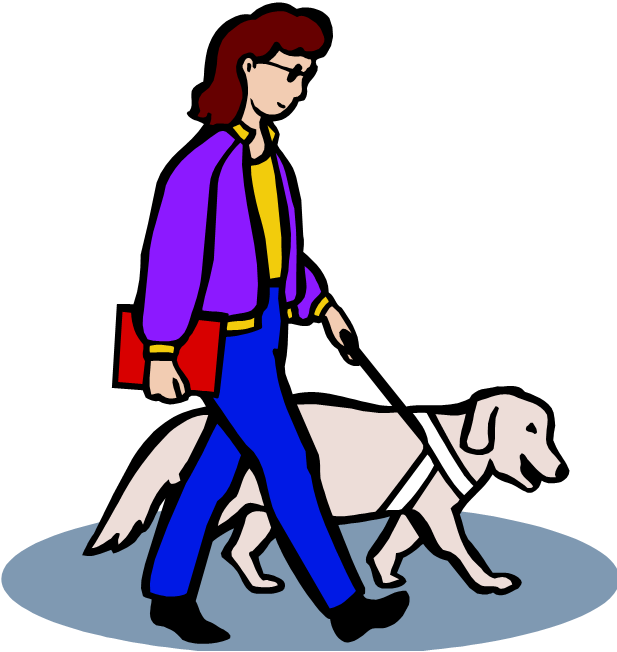
\includegraphics{images/guide_dog.png}
    \caption{Σκύλος οδηγός}
    \label{fig:guide-dog}
\end{figure}

\subsection{Ηλεκτρονικές συσκευές υποβοήθησης ταξιδιού (ETAs)}
Όσο η τεχνολογία προχωρούσε με ραγδαίους ρυθμούς και η υπολογιστική ισχύς γινόταν όλο και πιο μεγάλη, έκαναν την εμφάνισή τους οι λεγόμενες ηλεκτρονικές συσκευές υποβοήθησης ταξιδιού ή αλλιώς ΕΤΑs (Electronic Travel Aids). Αν και τα πρώτα χρόνια εμφάνισής τους οι ETAs επικεντρώνονταν κυρίως στην ανίχνευση και αποφυγή εμποδίων, τα τελευταία χρόνια έχουν αναπτυχθεί επαρκώς ώστε να υποστηρίζουν πλήρη περιγραφή των εμποδίων, της διαδρομής του χρήστη αλλά και συνεχή ανάδραση. Οι ερευνητές που ασχολούνται με την ανάπτυξη αυτών των συσκευών αξιοποιούν τις πληροφορίες που λαμβάνουν από το περιβάλλον γύρω από τον χρήστη και χρησιμοποιώντας συγκεκριμένες τεχνικές τον ειδοποιούν για τυχόν εμπόδια ή για την διαδρομή που πρέπει να ακολουθήσει.
\subsubsection{Αντίληψη περιβάλλοντος}
Οι άνθρωποι χρησιμοποιούν τα διάφορα αισθητήρια κανάλια για να κατανοήσουν το περιβάλλον γύρω τους. Όταν μιλάμε για πλοήγηση σε έναν χώρο τότε το κύριο αισθητήριο κανάλι που χρησιμοποιείται είναι αυτό της όρασης. Τα άτομα με μειωμένη ή καθόλου όραση τείνουν να αντικαθιστούν το οπτικό κανάλι με αυτό της ακοής ή της αφής. Συνήθως, το ακουστικό κανάλι είναι αυτό που χρησιμοποιείται κατά κύριο λόγο για να προσανατολιστούν και να αναγνωρίσουν τυχόν εμπόδια. Επιπρόσθετα, το απτικό κανάλι αξιοποιείται σε περίπτωση που τα άτομα αυτά θέλουν να κατανοήσουν με μεγαλύτερη λεπτομέρεια ένα εμπόδιο-αντικείμενο κοντά τους.

Επομένως, γίνεται κατανοητό ότι για να μπορέσουν οι ΕΤΑs να υποστηρίξουν τα άτομα με προβλήματα όραση πρέπει αρχικά να είναι σε θέση να αντιληφθούν το περιβάλλον γύρω τους με επιτυχία και ακρίβεια. Τον ρόλο των ματιών παίζουν οι διάφοροι τύποι αισθητήρων, όπως οι αισθητήρες υπερήχων, τα ραντάρ και οι κάμερες. Με χρήση αισθητήρων όπως αυτοί των υπερήχων το σύστημα είναι δυνατό να εντοπίσει ένα εμπόδιο μέχρι κάποια ορισμένη απόσταση, χωρίς ωστόσο να δώσει απάντηση σχετικά με την μορφολογία του. Από την άλλη μεριά, η χρήση κάμερας δίνει την δυνατότητα για πλήρη καταγραφή του περιβάλλοντος και με κατάλληλη επεξεργασία της εικόνας ή χρήση τεχνικών μηχανικής μάθησης μπορεί να δώσει απαντήσεις σχετικά με την μορφολογία των εμποδίων, την απόστασή τους, την υφή τους και το βέλτιστο μονοπάτι που μπορεί να ακολουθήσει ο χρήστης. Περισσότερα για τις κατηγορίες των συστημάτων πλοήγησης ανάλογα τον τρόπο "αίσθησης" του περιβάλλοντος θα αναλυθούν παρακάτω.
\subsubsection{Ανάδραση με χρήση ηχητικών ειδοποιήσεων}
Πέρα από την "αίσθηση" και την καταγραφή του περιβάλλοντος, ένα σύστημα πλοήγησης για άτομα με μειωμένη όραση θα πρέπει να μπορεί να μεταδώσει την οπτική πληροφορία στον χρήστη με αποδοτικό τρόπο. Επειδή όπως είπαμε και παραπάνω τα άτομα αυτά αξιοποιούν την αίσθηση της ακοής για τον προσανατολισμό τους τα περισσότερα ηλεκτρονικά συστήματα πλοήγησης χρησιμοποιούν το ακουστικό κανάλι για την μετάδοση της απαραίτητης πληροφορίας. Με άλλα λόγια, ο χρήστης ειδοποιείται μέσω ηχητικών σημάτων για την ύπαρξη κάποιου εμποδίου ή σε περίπτωση που υπάρχει ανάγκη για μια συγκεκριμένη δράση, όπως π.χ. να πραγματοποιήσει στροφή αριστερά/δεξιά ή να διασχίσει μια διάβαση πεζών. Τα ηχητικά αυτά σήματα μπορεί να είναι απλοί σύντομοι ή στιγμιαίοι ήχοι που ενημερώνουν τον χρήστη σχετικά με την απόσταση ενός εμποδίου, ή μπορεί να είναι σύντομες φράσεις/προτάσεις που να καθοδηγούν τον χρήστη σχετικά με την κατεύθυνση που πρέπει να ακολουθήσει.
\subsubsection{Ανάδραση με χρήση απτικών ειδοποιήσεων}
Πέρα από την ακοή, μια ακόμα αίσθηση που έχουν πολύ ανεπτυγμένη τα άτομα με προβλήματα όρασης είναι η αφή. Η αίσθηση της αφής είναι εκείνη που μας βοηθάει να αντιληφθούμε λεπτομέρειες σχετικά με τα αντικείμενα, όπως π.χ. την υφή των αντικειμένων. Τα τελευταία χρόνια έχει δοθεί ιδιαίτερη έμφαση στις συσκευές ΕΤΑs που βασίζονται στην ανάδραση με χρήση απτικών σημάτων, κυρίως επειδή ένα απτικό ερέθισμα είναι πολύ πιο διακριτικό σε σύγκριση με ένα ηχητικό και η αντίδραση του χρήστη σε αυτό είναι σχετικά πιο άμεση \cite{ng2012finger}. Οι διάφορες ETAs που έχουν κυκλοφορήσει κατά καιρούς χρησιμοποιούν ορισμένα μοτίβα δονήσεων για να ενεργοποιήσουν την αίσθηση της αφής στο χρήστη.



\section{Κατηγορίες συστημάτων υποβοήθησης πλοήγησης}
Η πλοήγηση ενός ατόμου μπορεί να διαιρεθεί σε δύο περιπτώσεις: α) πλοήγηση σε εσωτερικό χώρο, και β) πλοήγηση σε εξωτερικό χώρο. Και στις δύο περιπτώσεις για να έχουμε μια επιτυχημένη πλοήγηση είναι απαραίτητο να γνωρίζουμε τον προσανατολισμό που πρέπει να ακολουθήσει ο χρήστης, αλλά παράλληλα να ελέγχουμε ότι το μονοπάτι που ακολουθεί είναι ελεύθερο από εμπόδια. Συνεπώς, ένα ολοκληρωμένο σύστημα υποβοήθησης πλοήγησης για άτομα με μειωμένη όραση θα πρέπει να είναι σε θέση τόσο να παρέχει την κατεύθυνση του χρήστη σε σχέση με τον προορισμό του, όσο και να του εξασφαλίζει ένα ασφαλές μονοπάτι. 

Οι πρώτες συσκευές ETAs επικεντρώνονταν περισσότερο στο δεύτερο σκέλος, αυτό της αποφυγής εμποδίων, το οποίο επιτύγχαναν κυρίως με τη χρήση αισθητήρων υπερήχων ή σόναρ τα οποία εντόπιζαν ένα εμπόδιο σε μια συγκεκριμένη απόσταση και ειδοποιούσαν τον χρήστη για την ύπαρξη του. Με την ανάπτυξη της τεχνολογίας GPS (Global Positioning System) επήλθε και εντυπωσιακή πρόοδος όσον αφορά το πρώτο σκέλος των ETAs, αυτό της πλοήγησης. Το GPS λειτουργεί αξιοποιώντας την ύπαρξη 30+ δορυφόρων σε τροχιά γύρω από την γη, βάσει των οποίων μπορεί να εντοπίσει την τοποθεσία ενός δέκτη με ακρίβεια από μερικά μέτρα έως μερικά εκατοστά \cite{gps}. Η τεχνολογία αυτή επέτρεψε την κατασκευή συστημάτων πλοήγησης που όχι μόνο αναγνώριζαν πιθανά εμπόδια, αλλά μπορούσαν να κατευθύνουν τον χρήστη κατά την μετακίνησή του προς έναν προορισμό με αρκετά μεγάλη ακρίβεια. Ωστόσο, αν και το GPS λειτουργούσε αρκετά καλά στον εξωτερικό χώρο, η πλοήγηση στον εσωτερικό χώρο παρέμενε ακόμα ένα δύσκολο εγχείρημα, από την στιγμή που το σήμα του GPS εξασθενούσε σε μεγάλο βαθμό μέσα σε κτίρια. Για την αντιμετώπιση της πλοήγησης σε εσωτερικού χώρους έχουν δοθεί πολλαπλές λύσεις, με την πιο ενδιαφέρουσα από αυτές να αποτελεί η χρήση RFID (Radio Frequency IDentification), η οποία θα αναλυθεί παρακάτω. 

Τέλος, με την αύξηση της επεξεργαστικής ισχύος και την δυνατότητα κατασκευής όλο και μικρότερων επεξεργαστών τα συστήματα πλοήγησης, τόσο για εσωτερικούς όσο και για εξωτερικούς χώρους, άρχισαν πλέον να βασίζονται σε κάμερες και αισθητήρες βάθους. Παρακάτω παρουσιάζονται μερικά συστήματα πλοήγησης για άτομα με προβλήματα όρασης που έχουν αναπτυχθεί από προηγούμενες προσπάθειες ερευνητών. Έχει γίνει διαχωρισμός τους με βάση την τεχνολογία την οποία αξιοποιούν κατά κύριο λόγο για να πετύχουν την πλοήγηση του χρήστη ή την αναγνώριση των εμποδίων στην διαδρομή του.

\subsection{RFID}
Η τεχνολογία RFID, στα ελληνικά \textit{ταυτοποίηση μέσω ραδιοσυχνοτήτων}, αποτελεί την εξέλιξη των ραβδωτών κωδίκων barcode και χρησιμοποιείται ευρέως στην καθημερινή ζωή των ανθρώπων, κυρίως μέσω του εμπορίου. Ένα σύστημα RFID αποτελείται από δύο διαφορετικά μέρη:
\begin{enumerate}
    \item τον \textbf{πομποδέκτη}, οποίος συχνά αναφέρεται ως ετικέτα RFID (RFID tag) και
    \item τον \textbf{αναγνώστη ή αισθητήρα} (RFID reader).
\end{enumerate}

Ένα RFID tag αποτελείται από ένα εσωτερικό ολοκληρωμένο κύκλωμα το οποίο περιέχει μια κεραία για την επικοινωνία με τους RFID readers και μία μνήμη, στην οποία μπορούν να αποθηκευτούν διάφορα δεδομένα ή πληροφορίες για το αντικείμενο που φέρει την ετικέτα RFID. Ανάλογα την εφαρμογή στην οποία χρησιμοποιείται, η μνήμη μιας ετικέτας RFID μπορεί να είναι μόνο για ανάγνωση (\textit{Read Only Memory - ROM}), επανεγγράψιμη μνήμη (\textit{Read-Write Memory}), ή μνήμη μιας εγγραφής και πολλών αναγνώσεων (Write Once, Read Many - WORM) \cite{bonsor_fenlon_2007}.

\begin{figure}[H]
    \centering
    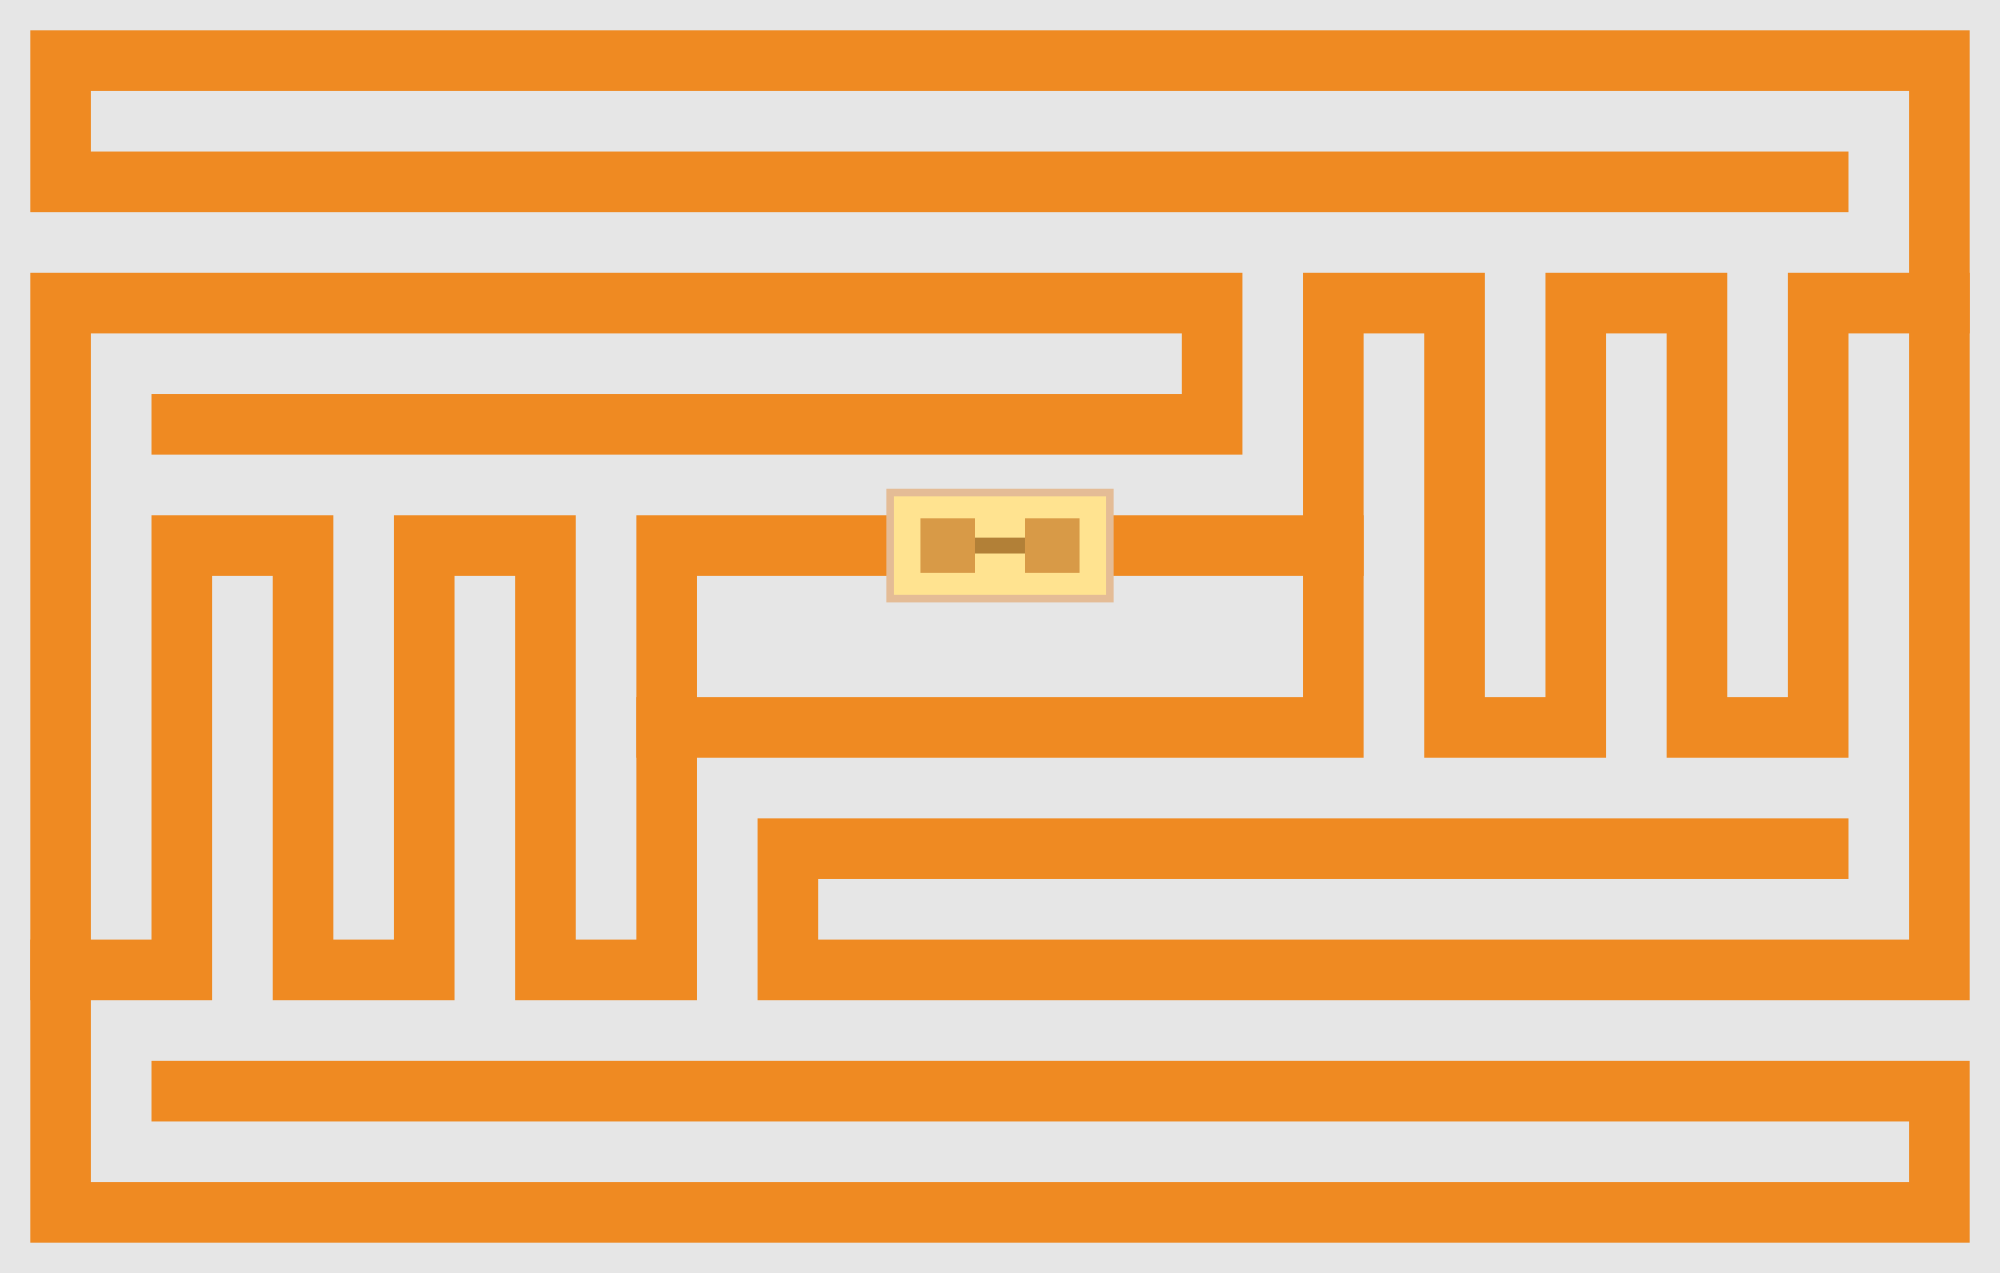
\includegraphics[width=0.4\textwidth]{images/rfid_tag.png}
    \caption{Παράδειγμα ολοκληρωμένου κυκλώματος ενός παθητικού RFID tag}
    \label{fig:rfid-tag}
\end{figure}

Αντίστοιχα, ένας RFID reader αποτελείται από μια κεραία, η οποία αναλαμβάνει την επικοινωνία με το RFID tag και μια μονάδα ελέγχου για την διαχείριση της ανταλλαγής δεδομένων με την εκάστοτε ετικέτα. Τα συστήματα RFID διακρίνονται σε ενεργητικά και παθητικά, ανάλογα με τον τρόπο επικοινωνίας της ετικέτας με τον αναγνώστη \cite{ElProCus_rfid, kaur2011rfid}. Στα ενεργητικά συστήματα οι ετικέτες τροφοδοτούνται αυτόνομα από μια εξωτερική πηγή τροφοδοσίας, όπως π.χ. μια μπαταρία, και έχουν την δυνατότητα να μεταδώσουν την πληροφορία τους σε μεγαλύτερες αποστάσεις. Αντίθετα, στα παθητικά συστήματα οι ετικέτες δεν έχουν δική τους πηγή τροφοδοσίας, αλλά λαμβάνουν την απαραίτητη ενέργεια από τους αναγνώστες RFID μέσω επαγωγικής σύζευξης κατά την φάση επικοινωνίας τους. Αν και τα παθητικά συστήματα έχουν πολύ μικρότερη εμβέλεια, αποτελούν την πλειοψηφία των RFID συστημάτων σήμερα και είναι αυτά που χρησιμοποιούνται σε εφαρμογές πλοήγησης για άτομα με μειωμένη όραση. Ένα τυπικό παράδειγμα λειτουργίας ενός τέτοιου συστήματος είναι η χρήση της πιστωτικής μας κάρτας κατά τη διάρκεια ανέπαφης συναλλαγής σε ένα κατάστημα. Η κάρτα μας παίζει τον ρόλο του RFID tag, ενώ η συσκευή POS του καταστήματος παίζει τον ρόλο του RFID reader. Μόλις η κάρτα βρεθεί αρκετά κοντά στο POS, λαμβάνει μέσω επαγωγικής σύζευξης την απαραίτητη ενέργεια από αυτό και τροφοδοτείται το ενσωματωμένο της ολοκληρωμένο κύκλωμα. Με αυτό τον τρόπο ενεργοποιείται ουσιαστικά η μετάδοση πληροφορίας, από την κάρτα προς το POS, η οποία πραγματοποιείται μέσω της κεραίας που υπάρχει και στα δύο μέρη.

\begin{figure}[H]
    \centering
    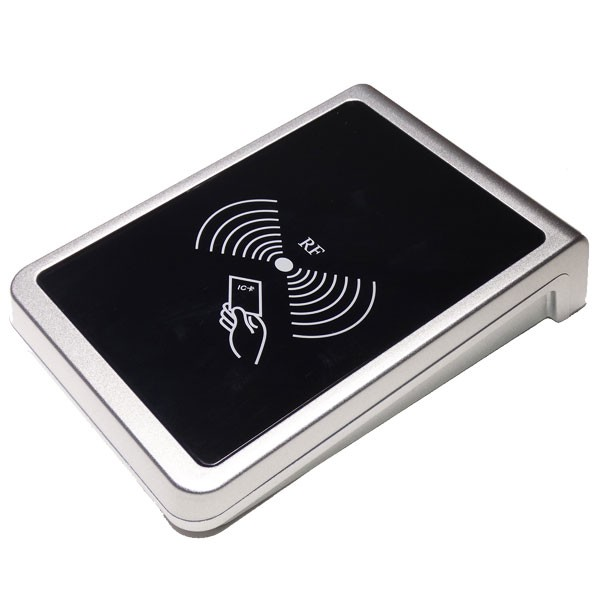
\includegraphics[width=0.4\textwidth]{images/rfid_reader.jpg}
    \caption{Παράδειγμα ενός RFID reader}
    \label{fig:rfid-reader}
\end{figure}

Η ενσωμάτωση των RFID συστημάτων σε συσκευές πλοήγησης για άτομα με προβλήματα όρασης αποτελεί μια έξυπνη λύση κυρίως σε εσωτερικούς χώρους, καθώς μπορούμε να τοποθετήσουμε πολλά RFID tags σε διαφορετικά σημεία-κόμβους μέσα στον χώρο, ή στο κτίριο που θέλουμε να καλύψουμε, ή ακόμα και κατά μήκος μιας διαδρομής που ακολουθούν τα άτομα με προβλήματα όρασης. Χρησιμοποιώντας έναν RFID reader τα άτομα αυτά θα είναι σε θέση να λαμβάνουν πληροφορίες σχετικά με την τοποθεσία στην οποία βρίσκονται και να καθοδηγούνται προς μια διαφορετική τοποθεσία, η οποία έχει ένα αντίστοιχο RFID tag.

Πραγματοποιώντας μια επισκόπηση της βιβλιογραφίας βρίσκουμε αρκετά συστήματα πλοήγησης που βασίζονται στην αξιοποίηση της τεχνολογίας RFID. Ένα αντιπροσωπευτικό παράδειγμα είναι αυτό που προτείνεται στο \cite{sammouda_mobile_2015}. Το προτεινόμενο σύστημα λειτουργεί σε εξωτερικούς και εσωτερικούς χώρους και αποτελείται από έναν RFID reader ενσωματωμένο στο λευκό μπαστούνι του χρήστη και πολλαπλά RFID tags διασκορπισμένα σε καίρια σημεία της διαδρομής του. Το σύστημα εντοπίζει την τοποθεσία του χρήστη είτε μέσω GPS, είτε μέσω ανάγνωσης του κοντινότερου RFID tag χρησιμοποιώντας τον ενσωματωμένο RFID reader. Σε περίπτωση που ο χρήστης θελήσει να κατευθυνθεί προς μια προκαθορισμένη τοποθεσία (π.χ. γραφείο, ή τουαλέτα) τότε το σύστημα τον προτρέπει να κινηθεί προς την σωστή κατεύθυνση, η οποία υπολογίζεται με χρήση ηλεκτρονικής πυξίδας, GPS και μέσω της ανάγνωσης του επόμενου RFID tag στο μονοπάτι του χρήστη. Πιο συγκεκριμένα, γίνεται σύγκριση της τωρινής θέσης του χρήστη σε σχέση με τον προορισμό και το κοντινότερο RFID tag και μέσω αυτής υπολογίζεται η κατάλληλη κατεύθυνση. Για να μπορεί λαμβάνει αξιόπιστες αποφάσεις το σύστημα διατηρεί μια βάση δεδομένων με όλες τις τοποθεσίες των τοποθετημένων RFID tags, συμπεριλαμβανομένων των αποστάσεων μεταξύ τους, οι οποίες ποικίλλουν από 4 έως 15 μέτρα.

\begin{figure}[H]
    \centering
    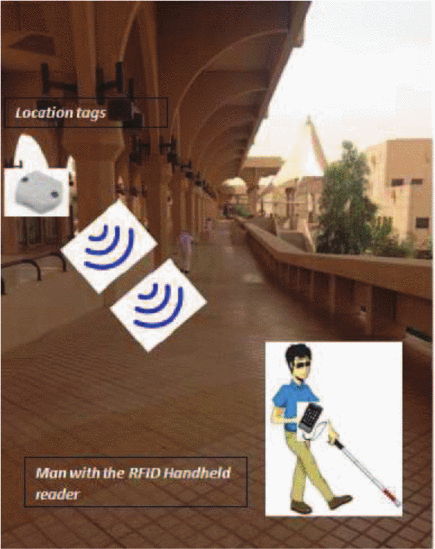
\includegraphics[width=0.6\textwidth]{images/rfid_paper.png}
    \caption{Περιγραφή του συστήματος που προτείνεται στο \cite{sammouda_mobile_2015}}
    \label{fig:sammouda_mobile}
\end{figure}
\hspace{1cm}

Παρατηρούμε ότι το παραπάνω σύστημα πετυχαίνει εν μέρει το σκοπό του, δηλαδή την καθοδήγηση του χρήστη προς ένα σημείο ενδιαφέροντος, αλλά γίνεται σαφές ότι ένα σύστημα πλοήγησης που βασίζεται σε RFID tags μπορεί να έχει ουσιαστικό νόημα μόνο σε εσωτερικούς χώρους ή σε συγκεκριμένες τοποθεσίες ενδιαφέροντος. Η ελεύθερη πλοήγηση του χρήστη μέσα σε μια πόλη δεν μπορεί να πραγματοποιηθεί, διότι σε αυτήν την περίπτωση θα απαιτούνταν ένας τεράστιος αριθμός από RFID tags κατά μήκος κάθε πιθανής διαδρομής του χρήστη!


\subsection{Learning-based}
Μια άλλη κατηγορία συστημάτων πλοήγησης είναι αυτή που βασίζεται στην αναγνώριση αντικειμένων/εμποδίων αξιοποιώντας τεχνικές της Μηχανικής Μάθησης (Machine Learning). Η βασική ιδέα πίσω από τέτοιου είδους συστήματα είναι ότι εκπαιδεύουμε έναν αλγόριθμο να αναγνωρίζει με πολύ μεγάλη ακρίβεια ένα αντικείμενο ή μια ομάδα αντικειμένων. Με άλλα λόγια, για να μπορέσει ο αλγόριθμος να εντοπίσει ένα συγκεκριμένο μοτίβο μέσα σε μια εικόνα, είτε αυτό είναι πρόσωπο, είτε είναι αντικείμενο, όπως π.χ. φανάρι, δρόμος κλπ, είναι απαραίτητο να έχει προηγηθεί μια διαδικασία "μάθησης", κατά την οποία παρέχουμε στον αλγόριθμο έναν πολύ μεγάλο αριθμό από γνωστές εικόνες που περιέχουν το μοτίβο που αναζητούμε. Ο αλγόριθμος λαμβάνει υπόψιν του όλες τις εικόνες που έχουν προηγηθεί και "δημιουργεί" ένα μοντέλο του αντικειμένου που θέλουμε να αναγνωρίζει. Αφού έχει επέλθει η διαδικασία της μάθησης το σύστημα είναι εκπαιδευμένο να αναγνωρίζει το συγκεκριμένο μοτίβο σε οποιαδήποτε άλλη νέα/άγνωστη εικόνα του δώσουμε ως είσοδο.

\begin{figure}[H]
    \centering
    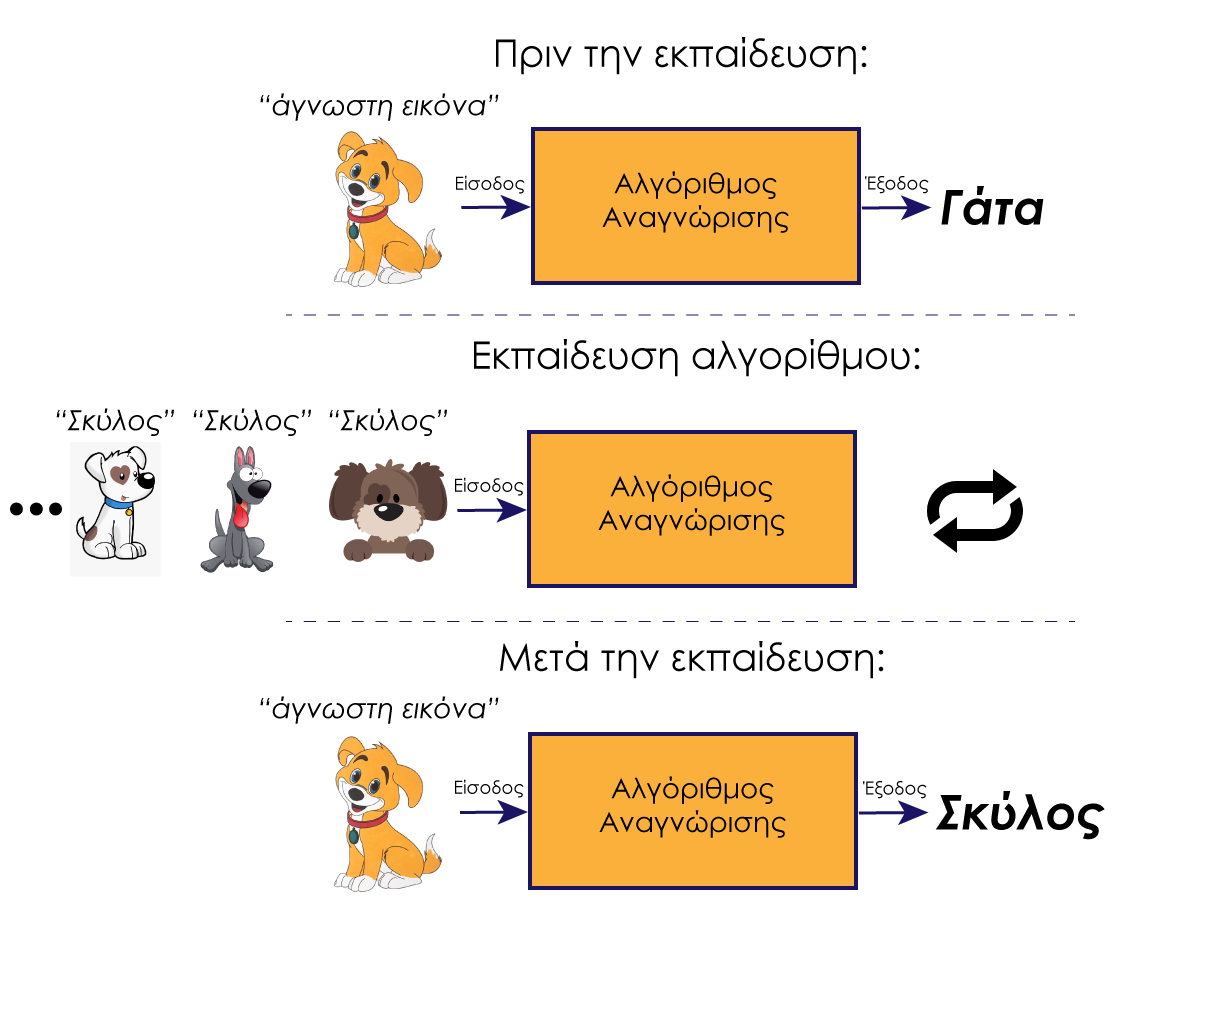
\includegraphics[width=0.8\textwidth]{images/learning_explained.png}
    \caption{Παράδειγμα εκπαίδευσης ενός αλγορίθμου μάθησης}
    \label{fig:learning-explained}
\end{figure}
\hspace{1cm}

Η εκπαίδευση αλγορίθμων για βελτιστοποιημένη αναγνώριση αντικειμένων δεν είναι μια νέα ιδέα στον τομέα της Υπολογιστικής Όρασης (Computer Vision), αλλά αποτελεί εξέλιξη της Αναγνώρισης Προτύπων (Pattern Recognition) η οποία μέχρι πρότινος χρησιμοποιούσε τις παραδοσιακές τεχνικές που σχετίζονται με την επεξεργασία εικόνας και σημάτων. Η ραγδαία αύξηση στην χρήση της μηχανικής μάθησης ως μέθοδο αναγνώρισης αντικειμένων συνέβη λόγω της αύξησης της διαθέσιμης επεξεργαστικής ισχύος τις τελευταίες δεκαετίες. Πλέον, ακόμα και ένα smartphone είναι ικανό να παρέχει επαρκή επεξεργαστική ισχύ για να εφαρμόσουμε μεθόδους μηχανικής μάθησης.

Οι εργασίες μηχανικής μάθησης χωρίζονται σε 3 (τρεις) μεγάλες κατηγορίες \cite{russell2016artificial} :

\begin{itemize}
    \item \textbf{Supervised Learning} (Επιβλεπόμενη Μάθηση): Ο αλγόριθμος μάθησης κατασκευάζει μια συνάρτηση που απεικονίζει τα δεδομένα εισόδου (σύνολο εκπαίδευσης) σε γνωστές επιθυμητές εξόδους. Η μάθηση χαρακτηρίζεται επιβλεπόμενη επειδή υπάρχει κάποιος "επιβλέπων" που παρέχει την σωστή τιμή εξόδου της συνάρτησης για το σύνολο εκπαίδευσης. Στόχος του αλγορίθμου είναι να "γενικεύσει" αυτήν την συνάρτηση, ώστε να μπορεί να προγνώσει με ακρίβεια την έξοδο του συστήματος σε δεδομένα εισόδου με αρχικά άγνωστη έξοδο. Μερικά παραδείγματα τεχνικών supervised learning είναι:
    \begin{itemize}
        \item Δέντρα Απόφασης (Decision Trees)
        \item Μάθηση Κανόνων (Rule Learning)
        \item Μάθηση κατά Περίπτωση (Instance Based Learning)
        \item Μάθηση κατά Bayes
        \item Γραμμική Παρεμβολή (Linear Regression)
        \item Νευρωνικά Δίκτυα (Neural Networks)
        \item Μηχανές Διανυσμάτων Υποστήριξης (Support Vector Machines)
    \end{itemize}
    
    \item \textbf{Unsupervised Learning} (Μη Επιβλεπόμενη Μάθηση):
    Ο αλγόριθμος αναλύει το σύνολο των δεδομένων εισόδου και κατασκευάζει ένα μοντέλο υπό μορφή συσχετίσεων ή ομαδοποιήσεων, χωρίς να γνωρίζει τις επιθυμητές εξόδους. Σαν αποτέλεσμα (έξοδος) προκύπτουν πρότυπα (περιγραφές), κάθε ένα από τα οποία περιγράφει ένα μέρος από τα δεδομένα. Τέτοιου τύπου αλγόριθμοι χρησιμοποιούνται κυρίως σε προβλήματα:
    \begin{itemize}
        \item Ανάλυσης Συσχετισμών (Association Analysis)
        \item Ομαδοποίησης (Clustering)
    \end{itemize}
    
    \item \textbf{Reinforcement Learning} (Ενισχυτική Μάθηση):
    Αποτελεί την πιο "αυτόνομη" μορφή αλγορίθμων μάθησης, όπου το σύστημα αλληλεπιδρά άμεσα με το περιβάλλον και μαθαίνει μια στρατηγική ενεργειών, που αποσκοπεί στην επίτευξη ενός στόχου, π.χ. οδήγηση ενός οχήματος. Χρησιμοποιείται κυρίως σε προβλήματα Σχεδιασμού (Planning), όπως για παράδειγμα ο έλεγχος κίνησης ρομπότ και η βελτιστοποίηση εργασιών σε εργοστασιακούς χώρους.
\end{itemize}

Στα συστήματα πλοήγησης χρησιμοποιείται κυρίως το supervised learning και πιο συγκεκριμένα εκπαιδεύονται Νευρωνικά Δίκτυα για την αναγνώριση του περιβάλλοντος.

\subsubsection{Νευρωνικά δίκτυα}
Ένα τεχνητό νευρωνικό δίκτυο - ΤΝΔ (Artificial Neural Network - ANN) στην μηχανική μάθηση είναι ένας αλγόριθμος εκμάθησης που εμπνέεται από τη δομή και τις λειτουργικές πτυχές των βιολογικών νευρωνικών δικτύων του ανθρώπινου εγκεφάλου. Με άλλα λόγια ο όρος "Νευρωνικά Δίκτυα" περιγράφει έναν αριθμό από διαφορετικά μαθηματικά μοντέλα που προσπαθούν να μιμηθούν τη συμπεριφορά των βιολογικών νευρώνων. Όπως τα νευρωνικά δίκτυα του εγκεφάλου περιέχουν έναν πολύ μεγάλο αριθμό από μεμονωμένα διακριτά στοιχεία, τους νευρώνες, έτσι και τα τεχνητά νευρωνικά δίκτυα αποτελούνται από έναν μεγάλο αριθμό απλών κόμβων (nodes) διασυνδεδεμένων μεταξύ τους, που παίζουν τον ρόλο των νευρώνων και οι οποίοι οργανώνονται σε στρώματα (layers). 
\begin{figure}[H]
    \centering
    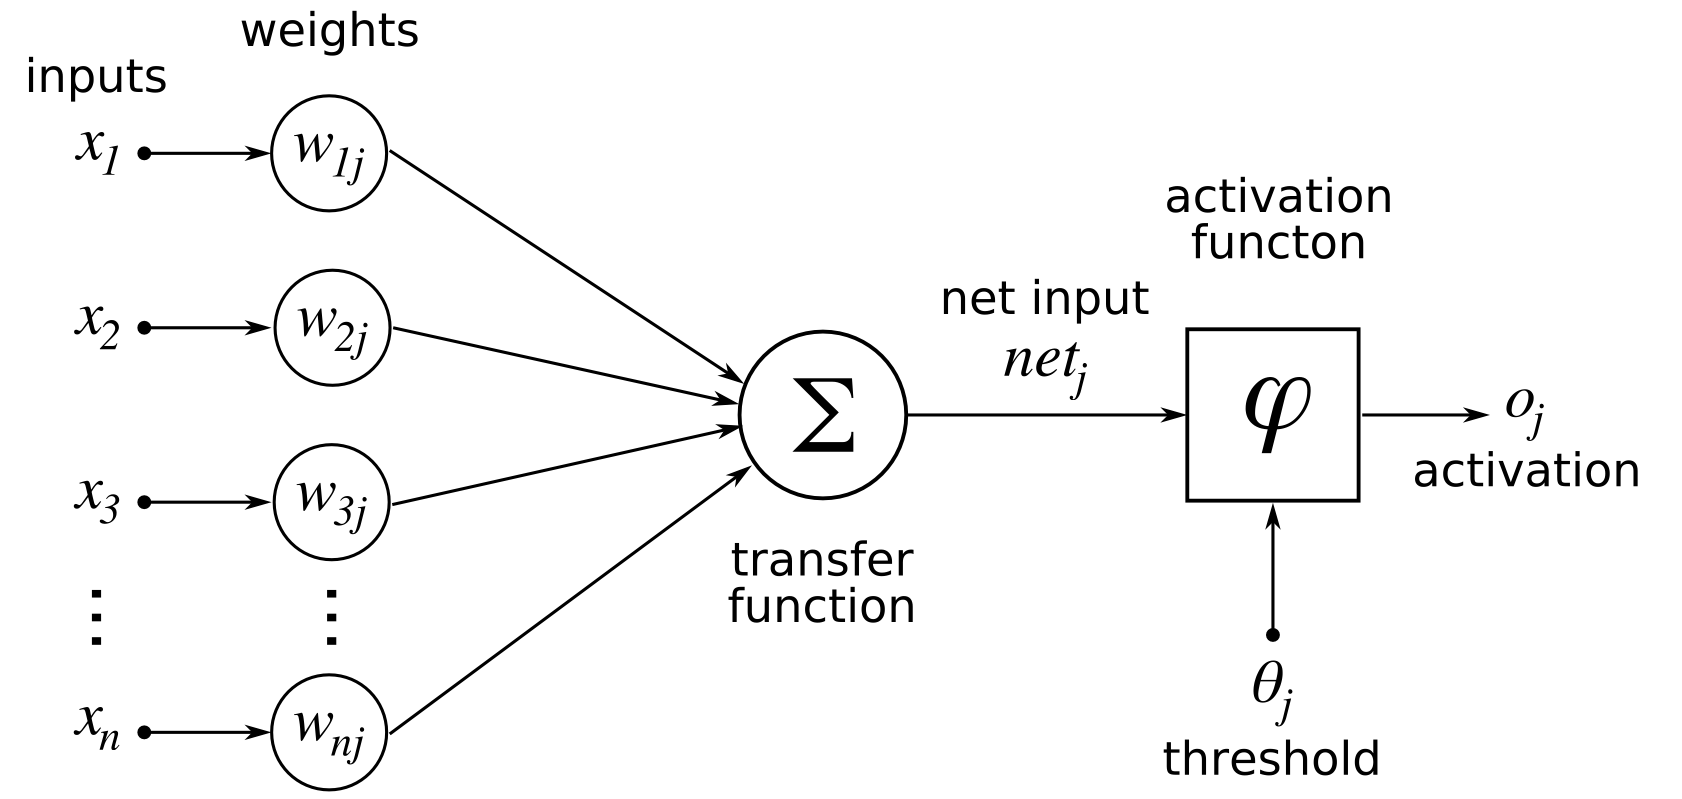
\includegraphics[width=0.6\textwidth]{images/art_neuron.png}
    \caption{Απεικόνιση λειτουργίας του απλούστερου τεχνητού νευρωνικού δικτύου, που ονομάζεται \textit{Perceptron} και αποτελείται από έναν μόνο νευρώνα}
    \label{fig:art-neuron}
\end{figure}
% \footnotetext{Chrislb (\url{https://commons.wikimedia.org/wiki/File:ArtificialNeuronModel\textunderscore english.png}), "ArtificialNeuronModel english", \url{https://creativecommons.org/licenses/by-sa/3.0/legalcode}}
\hspace{1cm}
Κάθε τεχνητός νευρώνας αποτελείται από πολλές εισόδους $x_i$ και μία μόνο έξοδο $y$. Κάθε είσοδος $x_i$ πολλαπλασιάζεται με ένα βάρος $w_i$ και αθροίζεται μέσω της συνάρτησης αθροίσματος (summation function) F, ως εξής: \[F = \sum_{i}^{n} x_i w_i\] Ο τεχνητός νευρώνας δίνει έξοδο μέσω της συνάρτησης ενεργοποίησης (activation function), μόνο όταν το σταθμισμένο άθροισμα $F$ είναι μεγαλύτερο μιας ορισμένης τιμής κατωφλίου (threshold value) $\theta$ \cite{Grossi2008}, δηλαδή όταν, \[\sum_{i}^{n} x_i w_i - \theta > 0\]

Το απλούστερο νευρωνικό δίκτυο Perceptron \cite{rosenblatt1961principles} (σχήμα \ref{fig:art-neuron}) αποτελείται από έναν μόνο νευρώνα και ένα επίπεδο. Συνήθως τα ΤΝΔ είναι πιο σύνθετα και οργανώνονται σε πολλαπλά επίπεδα (layers) τα οποία καλούνται και στρώματα. Τα ενδιάμεσα επίπεδα ονομάζονται κρυμμένα επίπεδα (hidden layers) και δεν είναι απαραίτητο να υπάρχουν. Οι κόμβοι-νευρώνες που υπάρχουν σε κάθε επίπεδο είναι συνδεδεμένοι μεταξύ τους, ώστε κάθε κόμβος-νευρώνας να έχει συνδέσμους με πολλούς άλλους κόμβους του ίδιου ή άλλου επιπέδου. Το δίκτυο δέχεται τις εισόδους $x_i$ στο επίπεδο εισόδου (input layer), το οποίο αλληλεπιδρά με τα κρυμμένα ενδιάμεσα επίπεδα, και παρέχει την έξοδό του μέσω του επιπέδου εξόδου (output layer).

\begin{figure}[H]
    \centering
    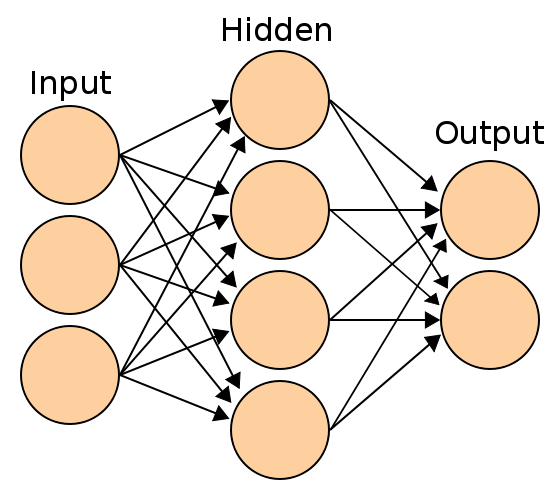
\includegraphics[width=0.4\textwidth]{images/ann_layers.png}
    \caption{Δομή επιπέδων σε ένα απλό τεχνητό νευρωνικό δίκτυο με ένα ενδιάμεσο κρυμμένο επίπεδο}
    \label{fig:ann-layers}
\end{figure}
% \footnotetext{en:User:Cburnett (\url{https://commons.wikimedia.org/wiki/File:Artificial\textunderscore neural\textunderscore network.svg}), "ArtificialNeuronModel english", \url{https://creativecommons.org/licenses/by-sa/3.0/legalcode}}

Σκοπός της παρούσας διπλωματικής εργασίας δεν είναι η αναλυτική περιγραφή των νευρωνικών δικτύων, γι'αυτό θα προχωρήσουμε κατευθείαν στην εφαρμογή τους όσον αφορά τα συστήματα πλοήγησης για άτομα με προβλήματα όρασης.

Η σημασία των νευρωνικών δικτύων στα συστήματα πλοήγησης σχετίζεται με την ακρίβεια που πετυχαίνουν στην αναγνώρισή αντικειμένων. Πιο συγκεκριμένα, τα τελευταία χρόνια χρησιμοποιούνται τα λεγόμενα Deep Neural Networks (Βαθιά Νευρωνικά Δίκτυα), τα οποία αποτελούνται από πολλά κρυμμένα επίπεδα και παρέχουν πολύ υψηλή ακρίβεια σε εφαρμογές όπως η αναγνώριση προσώπων, η κατηγοριοποίηση αντικειμένων κλπ. Ένα χαρακτηριστικό παράδειγμα αποτελεί το σύστημα που προτείνεται στο \cite{lin2017simple}, το οποίο χρησιμοποιεί την κάμερα από το smartphone του χρήστη και έναν υπολογιστή ως server. Το κύριο χαρακτηριστικό της συγκεκριμένης έρευνας είναι ότι, καθώς ο χρήστης πλοηγείται στον χώρο, το smartphone τραβάει φωτογραφίες από τον χώρο μπροστά από τον χρήστη και τις στέλνει, μέσω διαδικτύου, στον server όπου γίνεται η επεξεργασία τους. Πιο συγκεκριμένα, πριν την αποστολή της φωτογραφίας, γίνεται επιλογή των χαρακτηριστικών (feature selection) που θα χρησιμοποιηθούν ως είσοδοι στο νευρωνικό δίκτυο στην πλευρά του server. Ο server "τρέχει" δύο διαφορετικούς αλγορίθμους ταξινόμησης εικόνων, ανάλογα την ταχύτητα της διαδικτυακής σύνδεσης του χρήστη. Όταν η ταχύτητα σύνδεσης είναι υψηλή εφαρμόζεται ο αλγόριθμος Faster R-CNN (Faster Region-based Convolutional Neural Network), ενώ όταν η ταχύτητα σύνδεσης είναι αργή εφαρμόζεται ο αλγόριθμος YOLO (You Only Look Once). Αφού ο κάθε αλγόριθμος έχει εκπαιδευτεί να αναγνωρίζει και να ταξινομεί μια ομάδα αντικειμένων, το σύστημα αποστέλλει τα features, που έχουν εξαχθεί κατά τη διαδικασία του feature selection, στον server και αυτός με την σειρά του ταξινομεί την δοθείσα φωτογραφία. 

Όπως αναφέρεται και στην ίδια την έρευνα, αν και η χρήση των νευρωνικών δικτύων έχει ως αποτέλεσμα αρκετά υψηλή ακρίβεια, απαιτείται ιδιαίτερα υψηλή επεξεργαστική ισχύς, κάτι που δικαιολογεί και την χρήση του server ως εξωτερική μονάδα επεξεργασίας. Η χρήση του server και η αναγκαία μετάδοση των εικόνων από το smartphone προς αυτόν, συνεπάγεται την ύπαρξη μιας μικρής καθυστέρησης, η οποία μπορεί να γίνει σημαντικά μεγαλύτερη ανάλογα την ταχύτητα μετάδοσης και την πολυπλοκότητα του δικτύου που χρησιμοποιείται, έως ότου το σύστημα αποφανθεί για τον τύπο του εμποδίου που βρίσκεται μπροστά από τον χρήστη. Με άλλα λόγια, η έλλειψη επεξεργαστικής ισχύος οδηγεί σε προβλήματα όσον αφορά την real-time αναγνώριση αντικειμένων.

Καταλήγοντας, είναι αναγκαίο να τονίσουμε το γεγονός ότι τα βαθιά νευρωνικά δίκτυα αποτελούν πλέον μια πολύ αξιόπιστη λύση όσον αφορά τον εντοπισμό και την αναγνώριση εμποδίων σε συστήματα πλοήγησης, καθώς παρέχουν μεγάλα ποσοστά ακρίβειας και είναι σε θέση να αναγνωρίζουν ταυτόχρονα πολλαπλά αντικείμενα σε μια φωτογραφία. Από την άλλη πλευρά, όμως, ο περιοριστικός παράγοντας των υψηλών απαιτήσεων σε επεξεργαστική ισχύ και η αναγκαιότητα εκπαίδευσης των νευρωνικών δικτύων εκ των προτέρων, αποτελούν τροχοπέδη στην πλήρη αξιοποίησή τους και εφαρμογή τους σε φορητά συστήματα πλοήγησης για άτομα με μειωμένη όραση. Αξίζει, δε, να τονίσουμε ότι η εκπαίδευση των νευρωνικών δικτύων προϋποθέτει την ύπαρξη κατάλληλου σετ δεδομένων (dataset), για κάθε ξεχωριστό μοτίβο/αντικείμενο που θέλουμε να αναγνωρίζει το σύστημα, τα οποία δεν είναι πάντα διαθέσιμα. Αυτός είναι και ο λόγος που η παρούσα διπλωματική εργασία χρησιμοποιεί παραδοσιακές μεθόδους αναγνώρισης αντικειμένων, όπως αυτές που περιγράφονται παρακάτω.

\subsection{Vision-based}
Η κατηγορία αυτή των συστημάτων περιλαμβάνει τα συστήματα εκείνα που βασίζονται σε παραδοσιακές μεθόδους ανίχνευσης εμποδίων και αναγνώρισης αντικειμένων. Πιο συγκεκριμένα, η πλειοψηφία των συστημάτων πλοήγησης χρησιμοποιεί διάφορους αισθητήρες απόστασης, όπως αισθητήρες υπερήχων, LiDaR κλπ, για την ανίχνευση της ύπαρξης εμποδίου μπροστά από τον χρήστη. Παράλληλα, η ανίχνευση και η αναγνώριση του είδους των αντικειμένων γίνεται με μεθόδους ψηφιακής επεξεργασίας εικόνας. Παρακάτω αναλύεται η λειτουργία των βασικών αισθητήρων που εντοπίζονται σε ένα τέτοιο σύστημα.

\subsubsection{Ultrasonic sensors}
Η χρήση υπερήχων ανέκαθεν αποτελούσε μια από τις πιο γνωστές μεθόδους μέτρησης μικρών αποστάσεων και ανίχνευσης αντικειμένων, ενώ ακόμη και σήμερα αξιοποιούνται σε πολλές εφαρμογές, όπως είναι ο μη καταστροφικός έλεγχος (non destructive inspection) στη βιομηχανία ή η εξέταση υπερήχων στην απεικονιστική ιατρική. Ο άνθρωπος μπορεί να ακούσει ήχους σε ένα εύρος συχνοτήτων από 20 Hz έως 20 KHz (Σχήμα \ref{fig:ultrasound-range}). Οι υπέρηχοι είναι ηχητικά κύματα που έχουν συχνότητες μεγαλύτερες από 20 KHz, άρα δεν γίνονται αντιληπτοί από έναν φυσιολογικό άνθρωπο. Η σημασία των υπερήχων στην πλοήγηση και τον ηχο-εντοπισμό (echolocation) ανακαλύφθηκε για πρώτη φορά από τον Ιταλό Lazzaro Spallanzan, ο οποίος μελέτησε την συμπεριφορά των νυχτερίδων και παρατήρησε ότι προσανατολίζονται χρησιμοποιώντας υπερήχους και όχι όραση \cite{spallanzani1794lettere}. 

\begin{figure}[H]
    \centering
    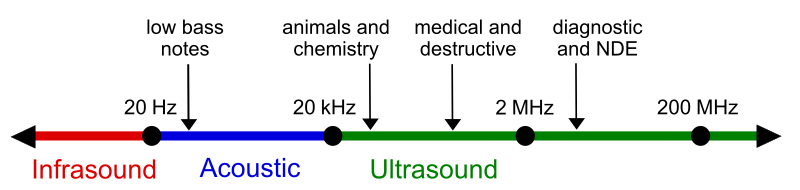
\includegraphics[width=0.6\textwidth]{images/Ultrasound_range_diagram.png}
    \caption{Διάγραμμα εύρους ηχητικών συχνοτήτων}
    \label{fig:ultrasound-range}
\end{figure}
\hspace{1cm}
% Ultrasound_range_diagram.png: The original uploader was LightYear at English Wikipedia. Ultrasound_range_diagram_png_(sk).svg: The original uploader was LightYear at English Wikipedia. derivative work: Coolth (talk) (https://commons.wikimedia.org/wiki/File:Ultrasound_range_diagram.svg), „Ultrasound range diagram“, https://creativecommons.org/licenses/by-sa/3.0/legalcode

Οι αισθητήρες υπερήχων αποτελούνται από έναν πομπό και έναν δέκτη υπερήχων και εκτιμούν την απόσταση ενός στόχου λαμβάνοντας υπόψη τους την αντανάκλαση ενός ραδιοκύματος ή ενός ηχητικού σήματος πάνω στο στόχο (Σχήμα \ref{fig:sonar-principle}). Για να το επιτύχουν αυτό χρησιμοποιούν τον χρόνο που έκανε το σήμα για να καλύψει την απόσταση από τον αισθητήρα στο αντικείμενο και πίσω. Η απόσταση ενός αντικειμένου μπροστά από τον αισθητήρα υπερήχου δίνεται ως εξής \cite{Theworki10:online}: \[distance = \frac{Time\textunderscore of\textunderscore Flight \times Speed\textunderscore of\textunderscore Sound}{2}\]

\begin{figure}[H]
    \centering
    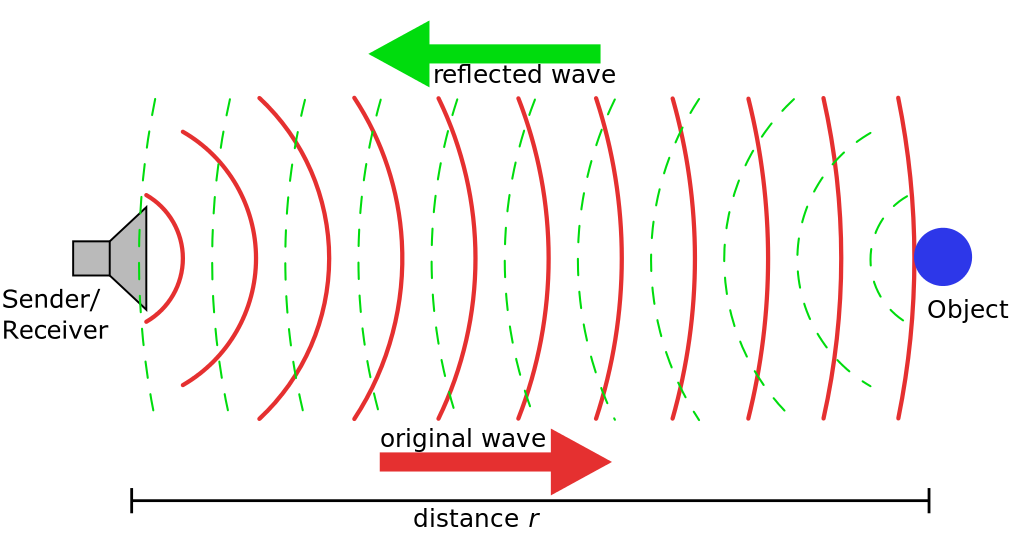
\includegraphics[width=0.6\textwidth]{images/Sonar_Principle.png}
    \caption{Αρχή λειτουργίας αισθητήρα υπερήχων}
    \label{fig:sonar-principle}
\end{figure}
\hspace{1cm}
% Georg Wiora (Dr. Schorsch) (https://commons.wikimedia.org/wiki/File:Sonar_Principle_EN.svg), „Sonar Principle EN“, https://creativecommons.org/licenses/by-sa/3.0/legalcode

Χάρη στην ευκολία χρήσης τους και το χαμηλό τους κόστος, πολλές εφαρμογές πλοήγησης αξιοποιούν τους αισθητήρες υπερήχων για να εντοπίζουν εμπόδια κατά μήκος του μονοπατιού του χρήστη. Ένα αντιπροσωπευτικό παράδειγμα αποτελεί η σχετική υλοποίηση στο \cite{bousbia2007ultrasonic}, όπου το προτεινόμενο σύστημα χρησιμοποιεί αποκλειστικά αισθητήρες υπερήχων για την καθοδήγηση του χρήστη. Χρησιμοποιώντας δύο αισθητήρες οι οποίοι εκπέμπουν παλμούς υπερήχων στα 40 KHz, είναι σε θέση να εντοπίζει συμπαγή αντικείμενα σε απόσταση 0.03 έως 6 μέτρα, και ανάλογα την εκτίμηση της απόστασης ειδοποιεί τον χρήστη μέσω δονήσεων.

\begin{figure}[H]
    \centering
    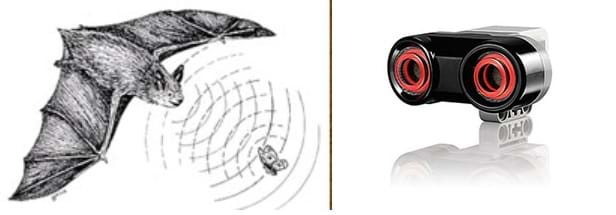
\includegraphics[width=0.6\textwidth]{images/ultrasonic_example.jpg}
    \caption{Αριστερά: Απεικόνιση του ηχο-εντοπισμού της νυχτερίδας. Δεξιά: Παράδειγμα ενός τυπικού αισθητήρα υπερήχων με έναν δέκτη και έναν πομπό.}
    \label{fig:sonar-example}
\end{figure}
\hspace{1cm}
% https://www.teachengineering.org/lessons/view/umo_sensorswork_lesson06
Αν και η χρήση υπερήχων λειτουργεί ικανοποιητικά σε εσωτερικούς χώρους, η αξιοποίησή τους σε εξωτερικά περιβάλλοντα έχει αρκετά μειονεκτήματα, κυρίως, λόγω της παρεμβολής από άλλα ηχητικά σήματα του ίδιου φάσματος. Επίσης, ένα μεγάλο μειονέκτημα αυτής της μεθόδου είναι η αδυναμία αναγνώρισης του είδους του αντικειμένου που ανιχνεύεται.

\subsubsection{LiDAR sensors}
Οι αισθητήρες Light Detection And Ranging, εν συντομία LiDAR, είναι συσκευές που λειτουργούν αξιοποιώντας το φως και την αντανάκλασή του πάνω σε επιφάνειες. Η αρχή λειτουργίας τους μοιάζει πολύ με εκείνη των αισθητήρων υπερήχων, μόνο που στην περίπτωση αυτή δεν εκπέμπουν υπερήχους, αλλά βασίζονται στην εκπομπή παλμικής ακτινοβολίας λέιζερ στην ατμόσφαιρα. Οι ακτίνες αντανακλούν πάνω στα αντικείμενα του περιβάλλοντος και ο αισθητήρας καταγράφει την ανακλώμενη ακτινοβολία λέιζερ, υπολογίζοντας την απόσταση των αντικειμένων ως εξής \cite{wwwlidar41:online}: \[distance = \frac{Time\textunderscore of\textunderscore Flight \times Speed\textunderscore of\textunderscore Light}{2}\]

Πιο συγκεκριμένα, οι αισθητήρες LiDAR εκπέμπουν ακτίνες φωτός στο υπεριώδες, στο ορατό, ή κοντά στο υπέρυθρο φάσμα ηλεκτρομαγνητικής ακτινοβολίας και είναι πολύ πιο ακριβείς από τους αντίστοιχους αισθητήρες υπερήχων, ενώ μπορούν επίσης να χρησιμοποιηθούν σε ένα μεγάλο εύρος υλικών, συμπεριλαμβανομένου μη-μεταλλικών αντικειμένων, βράχων, βροχής, ακόμα και σε μοριακό επίπεδο. Αυτή η μεγάλη ευελιξία των αισθητήρων LiDAR τους καθιστά πολύ χρήσιμους για την κατασκευή 3D αναπαραστάσεων των αντικειμένων-στόχων (3D reconstruction). Οι εφαρμογές τους περιλαμβάνουν την χρήση τους σε αεροφωτογραφίες, σε αυτόνομα οχήματα κ.α., ενώ αξίζει να τονίσουμε το γεγονός πως λειτουργούν καλύτερα σε εσωτερικά περιβάλλοντα, εξαιτίας την επίδρασης της υπέρυθρης ακτινοβολίας του ήλιου σε εξωτερικούς χώρους \cite{wiki:lidar}.

\begin{figure}[H]
    \centering
    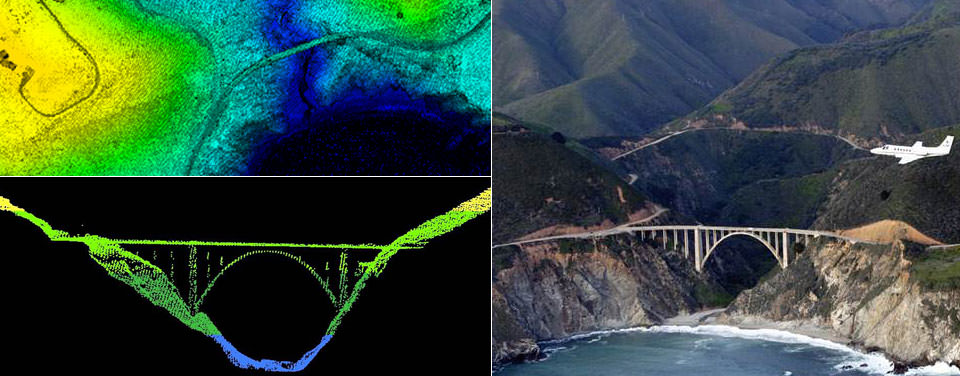
\includegraphics[width=0.8\textwidth]{images/lidar_3d_map.jpg}
    \caption{3D ψηφιακή αναπαράσταση μιας τοποθεσίας μέσω LiDAR}
    \label{fig:lidar-3dmap}
\end{figure}
\hspace{1cm}
% https://oceanservice.noaa.gov/facts/lidar.html
\begin{figure}[H]
    \centering
    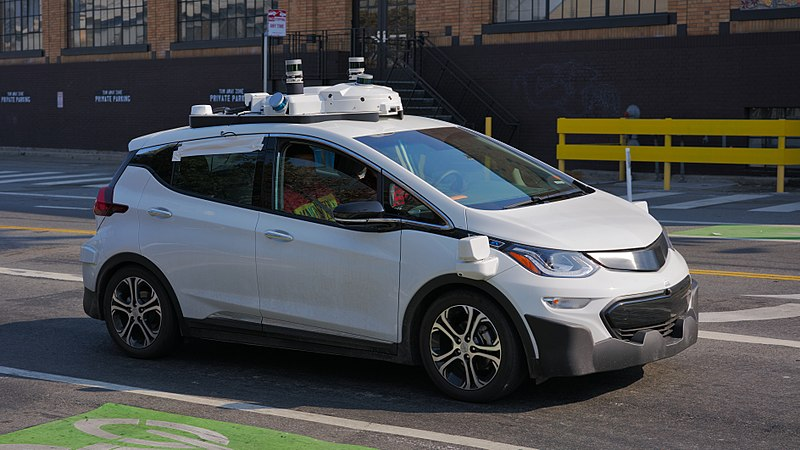
\includegraphics[width=0.6\textwidth]{images/lidar_car.jpg}
    \caption{Αισθητήρες LiDAR τοποθετούνται πάνω σε αυτόνομα οχήματα}
    \label{fig:lidar-car}
\end{figure}
\hspace{1cm}
% Dllu (https://commons.wikimedia.org/wiki/File:Cruise_Automation_Bolt_EV_third_generation_in_San_Francisco.jpg), https://creativecommons.org/licenses/by-sa/4.0/legalcode
Αν και η χρήση LiDAR δεν είναι τόσο διαδεδομένη σε φορητά συστήματα πλοήγησης, κυρίως, λόγω του όγκου τους και του υψηλού κόστους, υπάρχουν προσπάθειες που αναδεικνύουν την χρησιμότητά τους. Για παράδειγμα, στο \cite{miles2016lidar} προτείνεται ένα σύστημα πλοήγησης για άτομα με προβλήματα όρασης που βασίζεται αποκλειστικά στη χρήση ενός 2D LiDAR αισθητήρα (Σχήμα \ref{fig:lidar-example}), ο οποίος σκανάρει το περιβάλλον γύρω του σε ένα εύρος 270\degree και στέλνει τα δεδομένα σε μια μονάδα ψηφιακής επεξεργασίας σημάτων. Το αποτέλεσμα ανακοινώνεται στον χρήστη μέσω ηχητικών ειδοποιήσεων.
\begin{figure}[H]
    \centering
    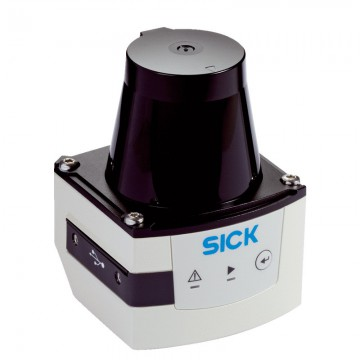
\includegraphics[width=0.4\textwidth]{images/lidar_example.jpg}
    \caption{Ο αισθητήρας LiDAR που χρησιμοποιείται στο \cite{miles2016lidar}}
    \label{fig:lidar-example}
\end{figure}
\hspace{1cm}

\subsubsection{RGB-D Camera}
Η πλειοψηφία των συστημάτων πλοήγησης για άτομα με προβλήματα όρασης χρησιμοποιεί κάμερες με ενσωματωμένο αισθητήρα βάθους, οι λεγόμενες RGB-D κάμερες. Τέτοια συστήματα είναι σε θέση τόσο να ανιχνεύουν τα εμπόδια μπροστά από τον χρήστη μέσω του αισθητήρα βάθους, όσο και να αναγνωρίζουν τον τύπο του εμποδίου, ή του αντικειμένου που μας ενδιαφέρει, μέσω της επεξεργασίας της RGB εικόνας που λαμβάνεται από την κάμερα.

Η πιο διαδεδομένη κάμερα με ενσωματωμένο αισθητήρα βάθους είναι η \textit{Microsoft Kinect RGB-D Camera}, η οποία πέρα από την αρχική της χρήση για το XBOX 360, αποτελεί την λύση σε πολλές πειραματικές προσπάθειες για ανάπτυξη φορητών συστημάτων πλοήγησης.
\begin{figure}[H]
    \centering
    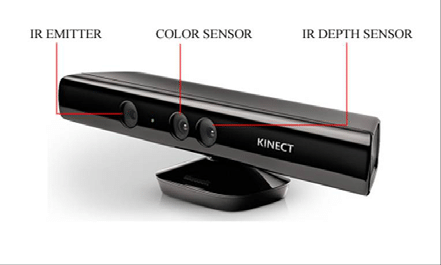
\includegraphics[width=0.6\textwidth]{images/kinect2.png}
    \caption{Ο αισθητήρας Kinect}
    \label{fig:kinect}
\end{figure}
\hspace{1cm}

Αυτοί οι αισθητήρες αποτελούνται συνήθως από έναν πομποδέκτη υπέρυθρης ακτινοβολίας (Infrared - IR) και έναν αισθητήρα RGB. Η αρχή λειτουργίας τους είναι η εξής: ο πομπός υπερύθρων προβάλλει στον χώρο ένα μοτίβο από σημεία υπέρυθρου φωτός (Structured Light technique) και ο δέκτης δέχεται τις ανακλώμενες ακτίνες. Το μοτίβο σημείων που εκπέμπεται παραμορφώνεται ανάλογα την επιφάνεια και τα αντικείμενα στα οποία ανακλάται. Στη συνέχεια γίνεται μια σύγκριση της αρχικής δομής των σημείων φωτός και αυτής που λήφθηκε από τον δέκτη. Έτσι, ανάλογα την παραμόρφωση που έχει υποστεί η δομή αυτή, παράγεται μια εικόνα βάθους, στην οποία κάθε pixel αντικατοπτρίζει την καρτεσιανή απόσταση (σε χιλιοστά) από την επιφάνεια της κάμερας μέχρι το κοντινότερο αντικείμενο στις συγκεκριμένες $x$,$y$ συντεταγμένες \cite{wiki:kinect}.
\begin{figure}[H]
    \centering
    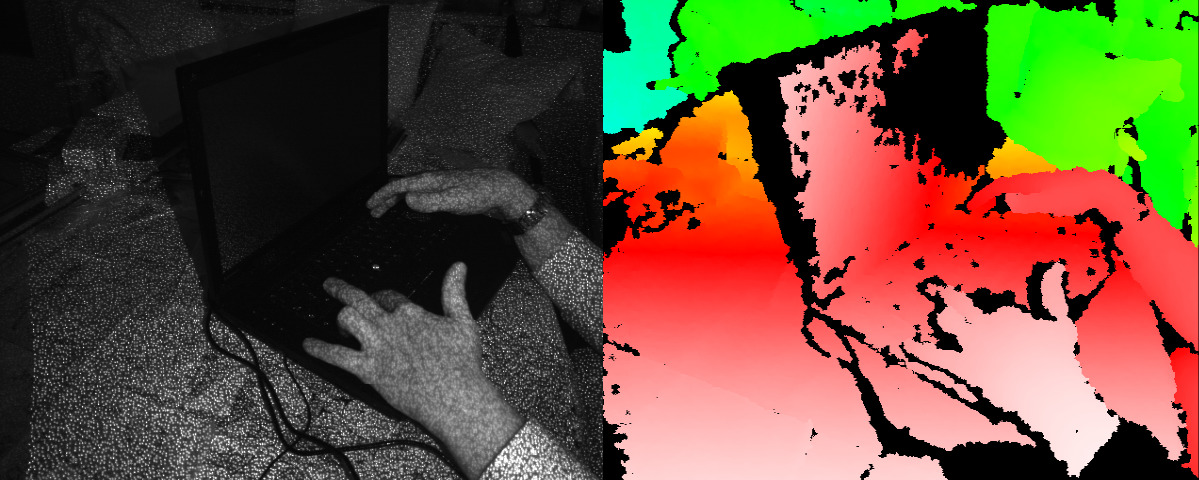
\includegraphics[width=\textwidth]{images/ir_structured_light.jpg}
    \caption{Αριστερά: Το μοτίβο από σημεία υπέρυθρου φωτός που εκπέμπεται. Δεξιά: Η παραγόμενη εικόνα βάθους ανάλογα με την παραμόρφωση της δομής του μοτίβου}
    \label{fig:structured-light}
\end{figure}
\hspace{1cm}

Ένα παράδειγμα συστήματος πλοήγησης για άτομα με προβλήματα όρασης, που χρησιμοποιεί τον αισθητήρα Kinect, είναι αυτό που προτείνεται στο \cite{kalaba2017}. Πιο συγκεκριμένα, παρουσιάζεται η δημιουργία ενός λειτουργικού, χαμηλού κόστους και διακριτικού συστήματος πλοήγησης, στο οποίο ο χρήστης φορά ένα γιλέκο με ένα ενσωματωμένο χωρικό πλέγμα από 16 κινητήρες δόνησης, που ενεργοποιούνται ανάλογα με τα εμπόδια που εντοπίζονται μπροστά από τον χρήστη. Η ανίχνευση των εμποδίων πραγματοποιείται μέσω του αισθητήρα Kinect.